\ifx \globalmark \undefined %% This is default.
	\documentclass[twoside,openright,11pt,a4paper]{report}

%\compiler avec xelatex
%\usepackage[applemac]{inputenc}
\usepackage[T1]{fontenc}
\usepackage[utf8]{inputenc} %latin1 est possible
%\usepackage[latin1]{inputenc} %latin1 est possible
\usepackage[francais]{babel}
\usepackage{lettrine}

\usepackage[text={13cm,20cm},centering]{geometry}

\renewcommand{\familydefault}{cmss}

\usepackage{graphicx}
\usepackage{amsmath}
\usepackage{amsfonts}
\usepackage{amssymb}
\usepackage{amsthm}
\usepackage{bm}
\usepackage{color}

\newcommand{\real}{\mathbb{R}}
\newcommand{\mb}{\mathbf}
\newcommand{\bos}{\boldsymbol}

\def \RR {I \! \! R}

\newcommand{\e}{\begin{equation}}  
\newcommand{\ee}{\end{equation}}
\newcommand{\eqn}{\begin{eqnarray}} 
\newcommand{\eeqn}{\end{eqnarray}} 
\newcommand{\eqnn}{\begin{eqnarray*}} 
\newcommand{\eeqnn}{\end{eqnarray*}} 

\newcommand{\bpm}{\begin{pmatrix}}
\newcommand{\epm}{\end{pmatrix}}

%\newcommand{\{\c c}}{\c c}

\newcommand{\bma}{\left(\begin{array}}
\newcommand{\ema}{\end{array}\right)} 
\newcommand{\hh}{\hspace{2mm}}
\newcommand{\hd}{\hspace{5mm}}
\newcommand{\hu}{\hspace{1cm}}
\newcommand{\vv}{\vspace{2mm}}
\newcommand{\vd}{\vspace{5mm}}
\newcommand{\vm}{\vspace{-2mm}}
\newcommand{\teq}{\triangleq}
%\newcommand{\qedb}{\,$\Box$}
\newcommand{\blanc}{$\left. \right.$}
\newcommand{\frts}[2]%
         {\frac{{\textstyle #1}}{{\textstyle #2}}}

\newcommand{\bindex}[3]%
{
\renewcommand{\arraystretch}{0.5}
\begin{array}[t]{c}
#1\\
{\scriptstyle #2}\\
{\scriptstyle #3}
\end{array}
\renewcommand{\arraystretch}{1}
}

\theoremstyle{definition}
\newtheorem{exemple}{{\bf Example}}[chapter]
\newtheorem{theoreme}[exemple]{{\bf Theorem}}
\newtheorem{propriete}[exemple]{{\bf Property}}
\newtheorem{definition}[exemple]{{\bf Definition}}
\newtheorem{remarque}[exemple]{{\bf Remark}}
\newtheorem{remarques}[exemple]{{\bf Remarks}}
\newtheorem{lemme}[exemple]{{\bf Lemma}}
\newtheorem{hypothese}[exemple]{{\bf Hypothesis}}
\newtheorem{exercice}{{\bf Exercise}}[chapter]

\newcommand{\xqedhere}[2]{%
 \rlap{\hbox to#1{\hfil\llap{\ensuremath{#2}}}}}

\newcommand{\xqed}[1]{%
 \leavevmode\unskip\penalty9999 \hbox{}\nobreak\hfill
 \quad\hbox{\ensuremath{#1}}}

\newcommand{\gf}{\fg\,\,}

\newcommand{\cata}[1] %
     {\renewcommand{\arraystretch}{0.5}
     \begin{array}[t]{c} \longrightarrow \\ {#1} \end{array}
     \renewcommand{\arraystretch}{1}}

\usepackage[isu]{caption}
%\usepackage[font=small,format=plain,labelfont=bf,up,textfont=it,up]{caption}
\setlength{\captionmargin}{60pt}

\newcommand{\cqfd}
{%
\mbox{}%
\nolinebreak%
\hfill%
\rule{2mm}{2mm}%
\medbreak%
\par%
}

\pagestyle{headings}

\renewcommand{\sectionmark}[1]{%
\markright{\thesection.\ #1}{}}

\renewcommand{\chaptermark}[1]{%
\markboth{\chaptername\ \thechapter.\ #1}{}}

\makeatletter 
\def\@seccntformat#1{\csname the#1\endcsname.\;} 
\makeatother

\title{ {\Huge {\textbf{Modélisation et analyse  \\ \vspace{4mm} des systèmes dynamiques }}} \\ \vspace{4cm} G. Bastin}

%\title{ {\Huge {\textbf{Modelisation et analyse  \\ \vspace{4mm} des systemes dynamiques }}} \\ \vspace{4cm} G. Bastin}


\date{\today}
	\begin{document} %% Crashes if put after (one of the many mysteries of LaTeX?).
\else 
	\documentclass{standalone}
	\begin{document}
\fi

\graphicspath{ {Chapitre8/images/} }

\setcounter{chapter}{7}
\chapter{Planar systems}
\chaptermark{Planar systems}\label{sysplans}


\lettrine[lines=1]{\bf W}{}ithin this chapter, we study in detail the behavior of 2D dynamical system trajectories (planar systems) when entry  $u(t)$ is constant~: $u(t)=\bar u$.  These systems are described by the following equations:
\eqnn
\dot x_1&=&f_1(x_1,x_2,\bar u),\\
\dot x_2&=&f_2(x_1,x_2,\bar u).
\eeqnn
A main motivation of this restriction to planar systems is to easily show the results representing the orbits in the phase plane, i.e. the plane of state variables $x_1$ and $x_2$. Besides, planar systems describe most of characteristic behaviors showing the difference between linear and nonlinear systems.
We will successively study the trajectories of linear systems, the behavior of nonlinear system trajectories near equilibrium points. We will focus on periodic trajectories and limit cycles. Finally, we will have an overview about bifurcation theory.

\section{Linear planar systems}

Let us consider planar systems when the entry $u(t)$ is constant~: 
$u(t)=\bar u$.
These systems are represented by the equation
$$\dot x=Ax +B \bar u,$$ where $A$ is a matrix
$2\times 2$. We assume there is at least an equilibrium state $\bar x$ corresponding to $\bar u$.

Thanks to a relevant state transformation, $z=M^{-1}(x-\bar x)$, we get $$\dot z=A'z$$ with
$$A'=M^{-1}AM.$$ 
The eigenvalues of $A'$ are the same ones than $A$ and  $A'$ has one of the following forms~:
\begin{itemize}
\item[{\bf a.}]
$$A'=\bma{cc} \lambda_1&0\\0&\lambda_2\ema$$ This form correspond to the case where $A$ has two distinct real eigenvalues $A$ or a double real eigenvalue with a geometric multiplicity  of 2. \\
\item[{\bf b.}]
$$A'=\bma{cc} \lambda&1\\0&\lambda\ema$$ This form corresponds to the case where 
 $A$ has  a double real eigenvalue of geometric multiplicity of 1. This is the ``Jordan form ''related to 
$A$. \\
\item[{\bf c.}]
$$A'=\bma{cc} \alpha&\beta\\-\beta&\alpha\ema,\;\;\; \beta >0$$ This form corresponds to the case where $A$ has two complex conjugate eigenvalues $\alpha\pm\beta i$. \\
\end{itemize} 

Thanks to these new coordinates, we are able to easily compute trajectories. They are described by the following equations :
\begin{itemize}
\item[{\bf a.}]
\eqnn
z_1(t)&=&z_1(0)e^{\lambda_1 t},\\
z_2(t)&=&z_2(0)e^{\lambda_2 t}.
\eeqnn 
\item[{\bf b.}]
\eqnn
z_1(t)&=&z_1(0)e^{\lambda t}+ t z_2(0)e^{\lambda t},\\
z_2(t)&=&z_2(0)e^{\lambda t}.
\eeqnn
\item[{\bf c.}]
\eqnn
z_1(t)&=&e^{\alpha t}(z_1(0)\cos \beta t+z_2(0) \sin \beta t),\\
z_2(t)&=&e^{\alpha t}(z_2(0)\cos \beta t-z_1(0) \sin \beta t).
\eeqnn
\end{itemize} 

The tables 8.1 à 8.3 show orbits as functions of one of these three forms and of the sign of eigenvalues. These orbits are represented in the plane $(z_1,z_2)$ and in the plane $(x_1,x_2)$, centered around the equilibrium point $(\bar x_1, \bar x_2)$.
In this second case, the directions in the figures correspond to the eigenvectors of the matrix $A$.

\begin{table}
\hspace*{-5mm}
\begin{eqnarray*}
\begin{array}{|c|c|c|l|}
\hline
\mbox{Type}&\mbox{Appearance of}& \mbox{Appearance of} &\mbox{Conditions}\\&&& \mbox{on the}\\
\mbox{of equilibrium}&\mbox{trajectories }(z_1,z_2)&\mbox{trajectories }(x_1,x_2)&
\mbox{eigenvalues}\\
\hline
\mbox{Attractive node} & & &\lambda_2 \leq \lambda_1 < 0\\
&\mbox{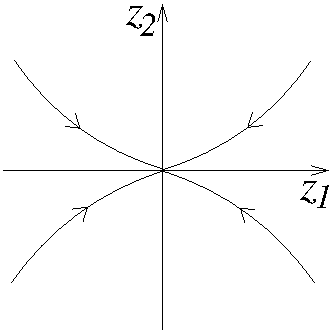
\includegraphics[width=25mm]{chap9taba1z}}&\mbox{\includegraphics[width=25mm]{chap9taba1x}} &\\
\hline
\mbox{Repulsive node}& & & 0<\lambda_1\leq\lambda_2 \\
&\mbox{\includegraphics[width=25mm]{chap9taba2z}}& \mbox{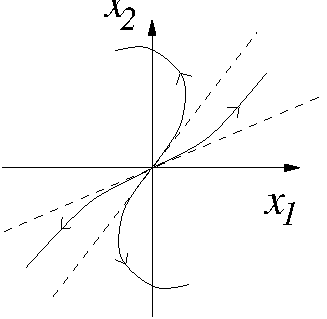
\includegraphics[width=25mm]{chap9taba2x}} &\\
\hline
\mbox{Saddle point} & & & \lambda_1 < 0 < \lambda_2 \\
&\mbox{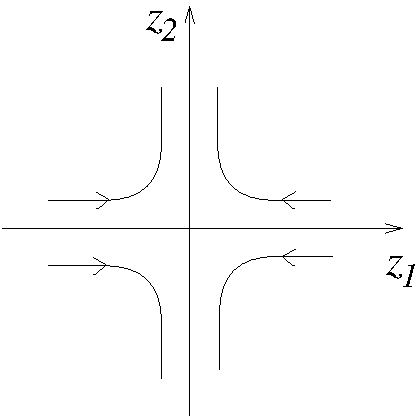
\includegraphics[width=25mm]{chap9taba3z}}& \mbox{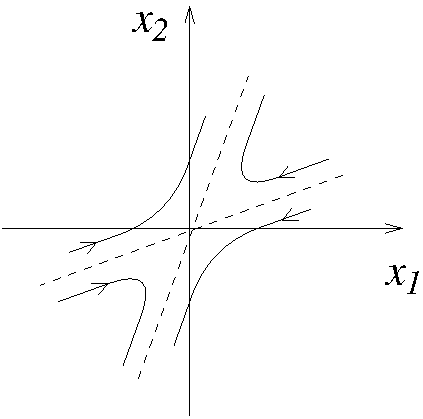
\includegraphics[width=25mm]{chap9taba3x}}&\\
\hline
\mbox{Non isolated} && &\lambda _1 = 0,  \\
\mbox{attractive equilibrium}&&&\lambda_2 < 0\\
&\mbox{\includegraphics[width=25mm]{chap9taba4z}}&\mbox{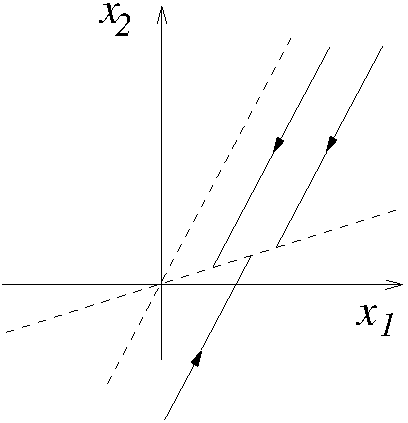
\includegraphics[width=25mm]{chap9taba4x}} &\\
\hline
\mbox{Non isolated} && &\lambda _1 = 0, \\
\mbox{repulsive equilibrium}&&& \lambda_2 > 0 \\
&\mbox{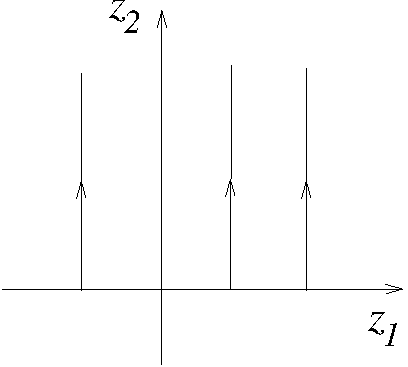
\includegraphics[width=25mm]{chap9taba5z}}& \mbox{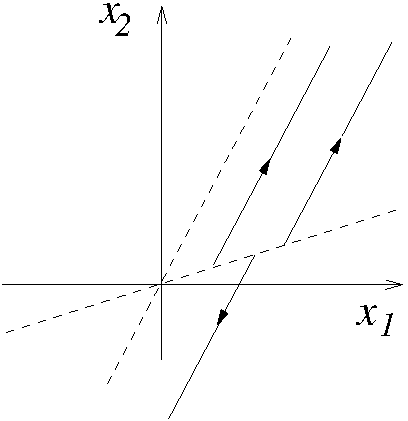
\includegraphics[width=25mm]{chap9taba5x}}&\\
\hline
\end{array}
\end{eqnarray*}
\caption{Orbits of linear planar systems~: case\;{\em \bf a.}}
\label{tablea}
\end{table}

\begin{remarques}{\hspace{1cm}}\end{remarques}
\begin{enumerate}
\item In the first two cases (see table~\ref{tablea}), when
$\lambda_1=\lambda_2$, the trajectories are straight and can be thus represented by a beam of lines coming from the origin.
\item If one of the eigenvalue is zero, the equilibrium is not isolated. The eigenvector corresponding to the eigenvalue zero defines a line of equilibrium points and all the trajectories are straight and converge to or come from a point of this line of equilibriums.
\end{enumerate}
\begin{table}
\begin{eqnarray*}
\begin{array}{|c|c|c|l|}
\hline
\mbox{Type}&\mbox{Appearance of}& \mbox{Appearance of} &\mbox{Conditions}\\&&& \mbox{on the}\\
\mbox{of equilibrium}&\mbox{trajectories }(z_1,z_2)&\mbox{trajectories }(x_1,x_2)&
\mbox{eigenvalues}\\
\hline
\begin{array}{l}
\mbox{Degenerated}\\
\mbox{attractive node}\end{array} & & &\begin{array}{l} \lambda = 0\\  \end{array} \mbox{(Jordan)} \\
&\mbox{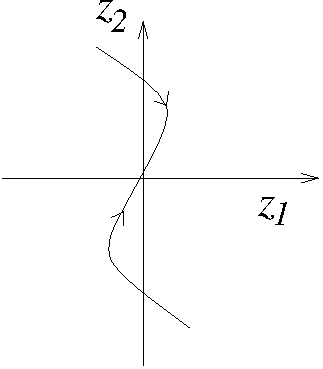
\includegraphics[width=30mm]{chap9tabB1z}}&\mbox{\includegraphics[width=30mm]{chap9tabB1x}} &\\
\hline
\begin{array}{l}
\mbox{Degenerated}\\   
\mbox{repulsive node}\end{array} & & & \begin{array}{l}\lambda >0 \\
\end{array}\mbox{(Jordan)}\\
&\mbox{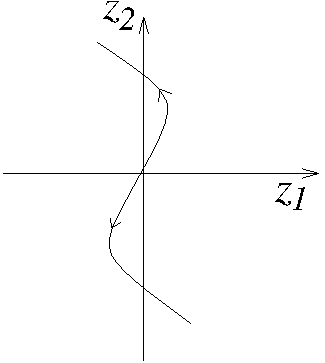
\includegraphics[width=30mm]{chap9tabB2z}}&\mbox{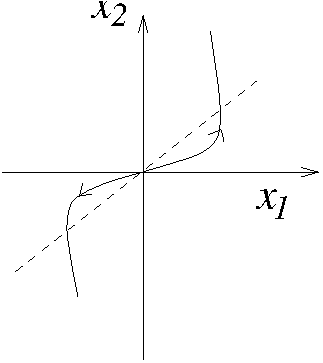
\includegraphics[width=30mm]{chap9tabB2x}} &\\
\hline
\begin{array}{l}
\mbox{Non isolated }\\   
\mbox{equilibrium}\end{array} & & & \begin{array}{l}\lambda=0\\
\end{array}\mbox{(Jordan)}\\
&\mbox{\includegraphics[width=30mm]{chap9tabB3z.jpg}}&\mbox{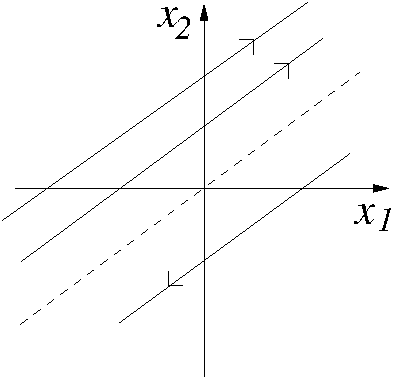
\includegraphics[width=30mm]{chap9tabB3x}} &\\
\hline
\end{array}
\end{eqnarray*}
\caption{Orbits of planar linear systems~: case\;{\em \bf b.}}
\label{tableb}
\end{table}
%inserer ici les remarques sur le cas b)
\begin{table}
\begin{eqnarray*}
\begin{array}{|c|c|c|l|}
\hline
\mbox{Type}&\mbox{Appearance of}& \mbox{Appearance of} &\mbox{Conditions}\\&&& \mbox{on the}\\
\mbox{of equilibrium}&\mbox{trajectories }(z_1,z_2)&\mbox{trajectories }(x_1,x_2)&
\mbox{eigenvalues}\\
\hline
\mbox{Attractive spiral} & & &\begin{array}{l}
\lambda_{1,2} = \alpha \pm \beta i\\
\alpha < 0 , \;\; \beta \neq 0 \end{array}\\
&\mbox{\includegraphics[width=30mm]
{chap9tabC1z}}&\mbox{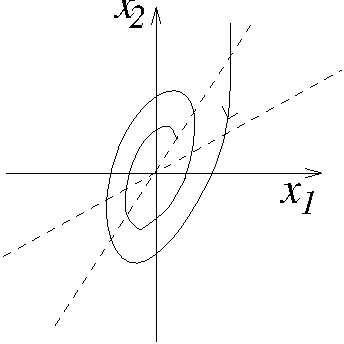
\includegraphics[width=30mm]{chap9tabC1x}} &\\
\hline
\mbox{Repulsive spiral} & & &\begin{array}{l}
\lambda_{1,2} = \alpha \pm \beta i\\
\alpha >0 , \;\; \beta \neq 0 \end{array}\\
&\mbox{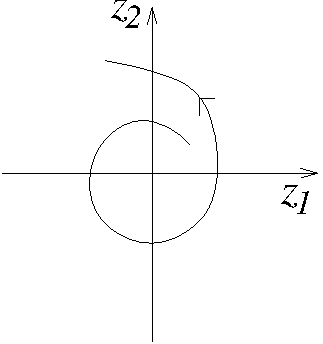
\includegraphics[width=30mm]{chap9tabC2z}}&\mbox{\includegraphics[width=30mm]{chap9tabC2x}} &\\
\hline
\mbox{Center} & & &\begin{array}{l}
\lambda_{1,2} = \pm \beta i\\
 \beta \neq 0 \end{array}\\
&\mbox{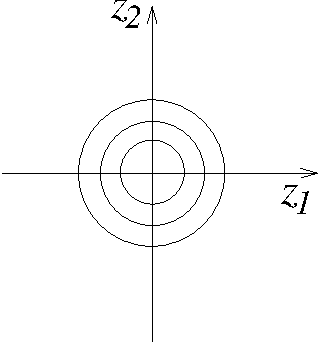
\includegraphics[width=30mm]{chap9tabC3z}}& \mbox{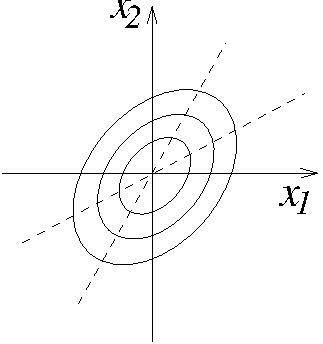
\includegraphics[width=30mm]{chap9tabC3x}}&\\
\hline
\end{array}
\end{eqnarray*}
\caption{Orbits of planar linear systems~: case\;{\em \bf c.}}
\label{tablec}
\end{table}
\renewcommand{\arraystretch}{1.0}

\begin{definition}{\em
When the equilibrium is such that the trajectories converge to this equilibrium, we say it is an attractive equilibrium.}\cqfd
\end{definition}

The eigenvalues $\lambda_1$ and $\lambda_2$ of matrix $A$ are the roots of the characteristic polynomial
\eqnn
p(x)&=&x^2-(\lambda_1+\lambda_2)x +\lambda_1 \lambda_2\\
&=&x^2-\mbox{tr}(A)x+\mbox{det}A.
\eeqnn
We observe that to determine the appearance of trajectories, it is not needed to compute explicitly these eigenvalues. Figure~\ref{fig:figlambda12}
show the nature of equilibrium (and thus the appearance of trajectories) as function of the two coefficients of characteristic polynomial that are respectively equal to the sum and product of eigenvalue.

\begin{figure}[htbp]
   \centering
   \includegraphics[width=12cm]{figlambda12} 
   \caption{
   Characteristics of equilibriums as function of the sum and product of eigenvalues.}
   \label{fig:figlambda12}
\end{figure}

We may wonder how the nature of these trajectories is sensitive to perturbations of the system. In order to answer to this question, we consider a nominal linear system $\dot x=
A x+Bu$ and a perturbation of the nominal system with the form $\dot x= (A+\Delta A) x+Bu$. If the matrix $A$ has distinct eigenvalues, we can show that they are continuously dependent of coefficients of $A$, which means that for every positive number
$\epsilon$, there exists a positive number $\delta$ such that if every coefficient of the perturbation $\Delta A$ is smaller than $\delta$, the eigenvalues of the perturbed matrix$A+\Delta A$ will be in the interior of balls of radius $\epsilon$ centered in the eigenvalues of $A$. Therefore, every eigenvalue is initially in the interior of the left  ($Re(\lambda)<0$) or right 
($Re(\lambda)>0$) half plane will stay in the same half plane for perturbations 
$\Delta A$ that are sufficiently small and, qualitatively, the trajectories of the perturbed system will look like to those of the nominal system~:
an attractive spiral stays an attractive spiral, a repulsive node stays a repulsive node, a saddle point stays a saddle point,... In this case, we say that such systems (or equilibriums) are {\em
structurally stable}. 

Unfortunately, this is not the same if the equilibrium corresponds to a  {\em center}. In this case, the systems has periodic elliptic trajectories and  pure imaginary eigenvalues. For this kind of systems, even small perturbation of the matrix $A$ can move out eigenvalues from imaginary axis. The corresponding trajectories become then attractive or repulsive spiral. A linear system having an equilibrium of center type is thus not structurally stable.

The case of linear system having one or two zero eigenvalues generally drives to a changement of property of trajectories under the effect of perturbations arbitrary small. When the system has a double eigenvalue that is different of zero, small perturbations can drive to real or complex conjugate eigenvalues, but the localisation within one of the half plane will not be changed. A degenerated attractive (repulsive) node can become an attractive (repulsive) node or an attractive (repulsive) spiral.

The previous analysis shows well that the imaginary axis can have some problems. We then introduce the following definition.

\begin{definition} \label{hyperbolique} 
If all the eigenvalues of $A$ have a non zero real part, the system
$\dot x=A x$ (or the equilibrium point)
is hyperbolic. \qed 
\end{definition}

Actually, an hyperbolic system is structurally stable and the trajectories will have the same properties with small perturbations. In the case of a double (non zero) eigenvalue, small perturbations can produce either a spiral, either a node; but the attractive or repulsive character  of the equilibrium will be preserved. Those observations have high value for the analysis of nonlinear systems.

 
 %Pierre-Alexandre's part ends here
%------------------------------------------------------------------------

 \section{Linéarisation des systèmes non linéaires}

Orbits illustrated in the table of the previous section are not only valid in the neighborhood of the point of equilibrium (returned to the origine). We characterized well thanks to these table all the possible orbits of the linear systems plans, whatever is the initial condition. This observation establishes a fundamental difference between linear and not linear systems. Indeed, we saw in the previous chapter that the non-linear systems can present several different isolated equilibrium for the same value of the entry $\bar u$. This implies that, contrary to the case of the linear systems, the behavior of orbits in the neighborhood of an equilibrium will keep most of the time a \textit{local character} and could never be expand to the whole plan of phase.
For this limitation, an important result allows however to extend to the non-linear systems a part of the analysis which we have just developed for the linear systems.


Set the dynamic system described by
\eqn
\dot x_1&=&f_1(x_1,x_2, \bar u),\label{f1}\\
\dot x_2&=&f_2(x_1,x_2, \bar u).\label{f2}
\eeqn
or, under condensed form,
\e \label{fxu}
\dot x=f(x,\bar u),
\ee for which we assumed the existence of an equilibrium $(\bar x,\bar u)$ such that $f(\bar x,\bar u)=0$.
 Assume further that the function $f(x,\bar u)$ is sufficiently regular in the neighborhood of this equilibrium for there allow a Taylor expansion convergent: 
 $$ \dot x = f(\bar{x}, \bar{u}) + \left ( \frac{\partial f(x, \bar{u})}{ \partial x}\right)_ {\bar x} {(x - \bar{x})} + \cdots . $$
The \textit{linear approximation} of this system at the neighborhood of the equilibrium
$(\bar x,\bar u)$, obtained by neglecting the terms of order greater or equal to 2 in the Taylor expansion of $f(x,\bar u)$ around $(\bar x,\bar u)$,
is given by
\e \label{approxli}
\dot {\tilde x} = \left ( {\frac{{\textstyle \partial f(x, \bar u)}}{{\textstyle \partial x}}} \right )_{\bar x} \tilde x 
\ee
where $\tilde x=x-\bar x$. Let $A=\left (\frac{\partial f(x, \bar u)}{\partial x}\right )_{\bar x}$, the Jacobian matrix of $f$ at equilibrium. We can then generalize the definition~\ref{hyperbolique} as follow~:
\begin{definition}\label{hyperbnl} {\bf{\em Hyperbolic equilibrium}}

The equilibrium $(\bar x,\bar u)$ of the non-linear systeme (\ref{fxu}) is said hyperbolic if all the eigen values of $A$ have a non-zero real part ($Re(\lambda_i(A))$ $ \neq 0, \forall i)$.\qed 
\end{definition}

It must be clear that it is the {\em equilibrium} $(\bar x,\bar u)$ which is (or which is not) hyperbolic, and not the non-linear system. Indeed, this system can have several isolated equilibrium for the same value $\bar u$, some being hyperbolic and others not. In which mesure the study of linear approxmation of a non-linear system at the neighborhood of an equilibrium allows to deduct the behavior of the non-linear system~? To specify what we understand by behavior, we want to be able to compare trajectories and then introduce the following definition.


\begin{definition} 
The trajectories (or orbits) of two dynamical systems are
{\em topologically equivalent} if it exists an {\em homeomorphism}
 (une bijection bicontinue) which allows to move from a trajectory of the first system to a trajectory of the second one. \qed
\end{definition} 

\begin{theoreme} {\bf{\em Hartman-Grobman, 1959}}

If the equilibrium $(\bar x,\bar u)$ is hyperbolic, then the trajectories of the non-linear system~(\ref{fxu})
{\em in a neighborhood of the equilibrium $(\bar x,\bar u)$} are topologically equivalent to the ones of the linear approximation~(\ref{approxli}). Specifically, it exists a neighborhood $X$ of $\bar x$, a neighborhood $\tilde{X}$ of $0$ and an homeomorphism $h: X \to \tilde{X}$ with $h(\bar x)=0$
such that if $t \mapsto x(t)$ is a trajectory of the non-linear-system~(\ref{fxu}) contain in $X$ (for a certain time interval), then $t \mapsto h(x(t))$ is a trajectory of the linear system (\ref{approxli}). \label{Hart}\qed
\end{theoreme}

Topologically equivalent trajectories have the same allure. So we can talk of node or attractive or repulsive center, or saddle, for the equilibrium of nonlinear systems by studying the eigenvalues of the linear approximation matrix, but {\bf no} center.

\begin{remarques}\hspace{10mm}\end{remarques}

\begin{enumerate}
\item The interest of this theorem is obvious. Its main limitation, its local character, is not less. In particular, this theorem doesn't give any indication about the size of the basin of attraction of an attrive equilibria.
\item In the case of a non-hyperbolic equilibrium, Dans le cas d'un {é}quilibre non hyperbolique, it is the higher order terms, those that have been neglected, that will determine the local behavior of trajectories.
\item The tools developed so far in this chapter are not specific to plan systems. Classification of linear systems, linearization, Hartman-Grobman theorem generalize without problems in any dimension
\item In the linearization~(\ref{approxli}), we keep $u=\bar u$ constant. We could also linearize $f$ around $u=\bar u$ to obtain a linearized type $\tilde{x}=A\tilde{x} + B\tilde{u}$. While $\tilde{u}=u-\bar u$ stay sufficiently small, and pour a sufficiently small interval of time, the trajectories of a non-linear and linear systems remain close, but there is no simple variation of the Hartman-Grobman theorem in this case.
\cqfd
\end{enumerate}



\section{Beyond plans systems}

The above considerations are not specific to plans systems.

The Hartman-Grobman theorem, for example, is true in any dimension $n \geq 2$, 
and classification of linear systems is similar. 

Consider a real matrix $A$ of arbitrary dimension.
If all its eigenvalues are distinct
then it can be diagonalized by real blocks $ 1 \ times $ 1
which contain a real eigenvalue, 
or $2 \times 2$, of the form $$\begin{pmatrix}
\alpha& \beta\\
-\beta& \alpha
\end{pmatrix},$$
 which encode a pair of conjugate eigenvalues $\alpha \pm \beta i$.
 
In this case the linear system (or linearised) can be described as direct product \footnote{A union of decoupled systems} of one-dimensional system or two-dimensional as seen in this chapter.



Briefly, the case of Jordan blocks is a little different and behaves as follows. A real Jordan block, for example

$$\begin{pmatrix}
\lambda& 1 & \\
       & \lambda & 1 \\
       &         & \lambda
\end{pmatrix}$$ 
generate a dynamic close to the two-dimentional case, linear combination of$e^{\lambda t}$, $te^{\lambda t}$, $t^2e^{\lambda t}$:

\eqnn
z_1(t)&=&z_1(0)e^{\lambda t}+ t z_2(0)e^{\lambda t}+ t^2 z_3(0)e^{\lambda t},\\
z_2(t)&=&z_2(0)e^{\lambda t}+ t z_3(0)e^{\lambda t},\\
z_3(t)&=&z_3(0)e^{\lambda t}.
\eeqnn

A Jordan block complex combines with its conjugate to form a block that looks eg like this:

\eqn
\begin{pmatrix}
\alpha & \beta & 1 & 0 \\
-\beta & \alpha&  0 & 1 \\
   &      &  \alpha & \beta\\
   &      &   -\beta & \alpha \\
\end{pmatrix}
\eeqn
The solutions then look like this:
\eqnn
z_1(t)&=&e^{\alpha t}(z_1(0)\cos \beta t+z_2(0) \sin \beta t+ t(z_3(0)\cos \beta t+z_4(0) \sin \beta t)),\\
z_2(t)&=&e^{\alpha t} (z_2(0)\cos \beta t-z_1(0) \sin \beta t+t(z_4(0)\cos \beta t-z_3(0) \sin \beta t)),\\
z_3(t)&=&e^{\alpha t}(z_3(0)\cos \beta t+z_4(0) \sin \beta t),\\
z_4(t)&=&e^{\alpha t}(z_4(0)\cos \beta t-z_3(0) \sin \beta t).
\eeqnn



Now illustrate the previous sections with some examples of non-linear 2nd order systems.



\subsection{Mechanical systems of one degree of
freedom}

The state equations of a mechanical system with one degree of freedom can be written (see chapter 2)~:
\begin{align*}
\dot x_1&=x_2,\\
m\dot x_2&=-g(x_1) -k(x_1)-h(x_2) + u,
\end{align*}
where $x_1$ 
is the coordinate position of the moving body, $x_2$ is the velocity, $m$ means the mass or inertia and $u$ represents a force or couple applied to an external system. Scalar functions $g(x_1)$ and $k(x_1)$ 
correspond to the gravity and elasticity while $h(x_2)$ (such that $h(0)=0$) represents the viscous friction. Dry friction is neglected. note also (see chapter~2, section~2.7) that 
\eqnn
g(x_1)+k(x_1) = \frac{\partial E_p}{\partial x_1}
\eeqnn
where $E_p$ refers to the potential energy of the system. 

The equilibria of the system are characterized by
\begin{align*}
\bar x_2 &= 0,\\
g(\bar x_1)+k(\bar x_1) &= \bar u.
\end{align*}
Without lost of generality, we consider the particular case where $m=1$. 
The Jacobian matrix of the system to equilibrium $(\bar x_1, 0,\bar
u)$ is written~: 
\eqnn
 A=\bma{cc} 0 & 1\\-\left (\frac{\partial^2E_p}{\partial x_1^2}\right
)_{\bar x_1} & -h'(0) \ema.
\eeqnn
The characteristic polynomial of the matrix is
\eqnn
p(x)=x^2+h'(0)x+\left (\frac{\partial^2E_p}{\partial x_1^2}\right )_{\bar
x_1}.
\eeqnn
 The product and the sum of the eigenvalues are given by
$$ \lambda_1\lambda_2=\left (\frac{\partial^2E_p}{\partial x_1^2}\right
)_{\bar x_1}, \;\;\; \lambda_1+\lambda_2=-h'(0).$$
The derivative $h'(0)$ the viscous friction is by nature non-negative~: $\lambda_1+\lambda_2 =-h'(0) \leq 0$.




The equilibria of the system are hyperbolic if
 \eqnn 
h'(0) >0 &\mbox{et }&  \left (\frac{\partial^2E_p}{\partial x_1^2}\right
)_{\bar x_1} \neq 0,\\
 \mbox{or if }  h'(0) =0 &\mbox{et }& \left (\frac{\partial^2E_p}{\partial x_1^2}\right
)_{\bar x_1} < 0.
\eeqnn
We observe that the equilibria are {\em not } hyoerbolics if potential energy $E_p(x_1)$ is a linear function of the position $x_1$, or more generally if the equilibrium corresponds to an inflection point $E_p(x_1)$. It's also the case when $h'(0)=0$ and $\left (\frac{\partial^2E_p}{\partial
x_1^2}\right )_{\bar x_1} \geq 0$.

Hyperbolic equilibria of a mechanical system with one degree of freedom can then be fully characterized as shown in table~\ref{tab:tabsysmec} (see also figure~\ref{fig:eqsysmec}).
\begin{figure}[t] 
   \centering
   \includegraphics[height=4cm]{eqsysmec} 
   \caption{Eigenvalues location of equilibria of a mechanical system with one degree of freedom}
   \label{fig:eqsysmec}
\end{figure}
\begin{table}
\hspace*{5mm}
%\renewcommand{\arraystretch}{1.2}
\begin{tabular}{|c|c|}
\hline
Characterization&Nature of hyperbolic equilibria\\ \hline
{}&{}\\
$0< [h'(0)]^2 <4 \left (\frts{\partial^2E_p}{\partial x_1^2}\right
)_{\bar x_1}$&stable center \\
{}&{}\\ \hline
{}&{}\\
$0<4 \left (\frts{\partial^2E_p}{\partial x_1^2}\right
)_{\bar x_1}\leq [h'(0)]^2$&stable node \\
{}&{}\\
 \hline
 {}&{}\\
$\left (\frts{\partial^2E_p}{\partial x_1^2}\right
)_{\bar x_1} <0$&csaddle \\ 
{}&{}\\
\hline
\end{tabular}
\caption{
Hyperbolic equilibria of mechanical systems with one degree
freedom}
\label{tab:tabsysmec}
\end{table}
In particular, we observe that an hyperbolic equilibrium can never be a node or a repulsive center.

\subsection{Les circuits électriques RLC}

The simple electrical circuits containing only inductance and capacitance are generally referred to {\em RLC circuits} in the literature. In reference books
Electrical Engineering or circuit theory, they are subject
to a thorough study because they constitute the basic configuration of many practical devices (filters, oscillators, ...).

The {\em RLC series circuit shown in Figure~\ref{fig:RLCs}
is a tipical example.
\begin{figure}[htbp] 
   \centering
   \includegraphics[height=2.5cm]{RLCs} 
   \caption{RLC series circuits}
   \label{fig:RLCs}
\end{figure}
Applying the principles discussed in chapter~3, the dynamic behavior of this circuit is described by a model
of 2-dimensional state~:
\eqnn
L \dot x_1&=&-r(x_1)-x_2 +u\\
C \dot x_2&=&x_1
\eeqnn
where $x_1=i$ is the current in the linear inductance $L$, $x_2=v$ is the voltage across the linear capacity $C$ and $r(x_1)$ is the voltage-current characteristic (eventually non-linear)
of the resistance.
\begin{figure}[t] 
   \centering
   \includegraphics[height=4cm]{figrlc} 
   \caption{Eigenvalues location of equilibria of a RLC circuit}
   \label{fig:figrlc}
\end{figure}

The equilibria of the system are characterized by the equations~:
\begin{align*}
\bar x_2 +r(0) &= \bar u,\\
\bar x_1 &= 0.
\end{align*}
Without loss of generality, consider the special case $L=1$ and $C=1$. 
The Jacobian matrix of the system to equilibrium $(0,\bar x_2,\bar u)$ is written~:
$$A=\bma{cc} -r'(0) & -1\\1&0\ema .$$
The characteristic polynomial of the matrix is~:
\eqnn
p(x)&=&\lambda^2+r'(0) \lambda +1\\
\mbox{o{ù} }\;\; r'(0)&\triangleq&(\partial r/\partial x_1)_{x_1=0}.
\eeqnn
The product and the sum of the eigenvalues are given by
$$ \lambda_1\lambda_2=1,  \;\;\; \lambda_1+\lambda_2=-r'(0).$$
The equilibria of the system are hyperbolic if $r'(0)\neq 0$, 
i.e. if the derivative of the characteristic of the resistance is not
zero at the origin. We observe that this is especially the case for
linear resistance.

Hyperbolic equilibria of a series RLC circuit are then completely characterized as indicated in table \ref{tabrlc} 
(see also figure~\ref{fig:figrlc}).
\begin{table}
\centering
\renewcommand{\arraystretch}{3.0}
\begin{tabular}{|c|c|}
\hline
&Nature of hyperbolics equilibria\\ \hline
$r^{'}(0) \geq 2$&attractive node \\ \hline
$0 < r^{'}(0) < 2$&attractive center \\ \hline
$-2 < r^{'}(0) < 0$&repulsive center \\ \hline
$r^{'}(0) \leq -2 $& repulsive node\\
\hline
\end{tabular}
\caption{Hyperbolic equilibria of an RLC circuit}\label{tabrlc}
\end{table}
In particular we note that a hyperbolic equilibrium of a series RLC circuit can never be a saddle.

\subsection{Systems with two compartments}

Consider two compartments systems whose graph is shown in figure~\ref{fig:deuxcomp}.
\begin{figure}[htbp] 
   \centering
   \includegraphics[height=4cm]{deuxcomp} 
   \caption{Système à deux compartiments}
   \label{fig:deuxcomp}
\end{figure}
The input signal $u$ is the first compartment volumetric flow rate. We assume that the flows exchanged between the compartments meet the modeling conditions
$C1 - C4$ of chapter 4 (Section 4.3).  The dynamics of the system is then described by a two dimensional state model of the general form:
\eqnn
\dot x_1 &=& -q_{12} (x_1, x_2) + q_{21} (x_2,x_1) - q_{10} (x_1) + u\\
\dot x_2 &=& q_{12}(x_1,x_2)-q_{21} (x_2,x_1) - q_{20} (x_2)
\eeqnn
The functions $q_{ij}$ satisfy the following conditions on the positive orthant :
\e
q_{ij}(0, x_j) = 0 \;\;\; \frac{\partial q_{ij}}{\partial
x_{i}} \geq 0 \;\; \frac{\partial q_{ij}}{\partial
x_{j}} \leq 0 \label{orthpositif}
\ee
Under these conditions, the system has an infinite number of isolated positive equilibria
$(\bar x_1, \bar x_2, \bar u)$.  The Jacobian matrix around one of these equilibria is written :
$$
A = \bma{cc} -(a+c) &  b\\a & -(b+d) 
\ema
$$
with the following simplified notation (all the partial derivatives are measured at equilibrium state ) :
\eqnn
a &\triangleq & \frac{\partial q_{12}}{\partial x_1} - \frac{\partial
q_{21}}{\partial x_1} \hspace*{15mm}c \triangleq \frac{\partial q_{10}}{\partial x_1}\\
b &\triangleq & \frac{\partial q_{21}}{\partial x_2} - \frac{\partial
q_{12}}{\partial x_2} \hspace*{15mm} d \triangleq \frac{\partial q_{20}}{\partial x_2}
\eeqnn
Under the conditions (\ref{orthpositif}), we immediately observe that
$a,b,c,d, \geq~0$.  The characteristic polynomial of the Jacobian matrix is:
$$
p(x) = x^2 + (a+b+c+d)x + (ad+bc+cd)
$$
The product and the sum of the eigenvalues are given by:
$$
\lambda_1 \lambda_2 = ad+bc+cd \;\;\;\; \lambda_1 + \lambda_2 = -(a+b+c+d)
$$
The equilibria of the system are hyperbolic if the following inequalities are satisfied:
$$
a+b+c+d > 0 \;\;\mbox{ et }\;\; ad+bc+cd > 0
$$

It is easy to show that, under these conditions, the following inequality is satisfied:
$$
0<4 (ad+bc+cd) \leq (a+b+c+d)^2
$$
We deduce that hyperbolic equilibrium of a two-compartments system may be only attractive nodes (see figure~\ref{fig:eq2comp}).
\begin{figure}[htbp] 
   \centering
   \includegraphics[height=4cm]{eq2comp} 
   \caption{Eigenvalues location of equilibria of a two-compartment system}
   \label{fig:eq2comp}
\end{figure}

\subsection{Les systèmes réactionnels à deux espèces}


The simplest reaction systems involve two species. For example this is the case of an irreversible reaction converting a reagent
$X_1$ in a product $X_2$ :
$$
X_1 \longrightarrow X_2
$$
Assume that this reaction takes place in a continuous reactor perfectly mixed with constant volume. The reactor is fed with the species
 $X_1$, at strictly positive constant volumetric flow rate. As we saw in Chapter 5, the reactor state model can be written as follows:
\eqnn
\dot x_1 &=& -r(x_1,x_2) + d(u-x_1)\\
\dot x_2 &=& r(x_1,x_2) - dx_2
\eeqnn
where  $x_1$ et $x_2$ represent the concentrations of the species $X_1$ and $X_2$ in the reactional environment, $d$ is the rate of dilution in the reactional environment and $u$ is the concentration of the reagent $X_1$ in the diet. The reaction kinetics $r(x_1,x_2)$ is assumed to be a function of the concentrations of the two species.
\begin{figure}[t] 
   \centering
   \includegraphics[height=4cm]{fig2esp} 
   \caption{Eigenvalues location of the equilibria of a two species reactional system}
   \label{fig:fig2esp}
\end{figure}

The equilibria of the system are characterized by the equations:
$$
d\bar x_2 = d(\bar u-\bar x_1) = r(\bar x_1, \bar x_2)
$$
These equations involve at the equilibrium $\bar x_1 + \bar x_2 = \bar u$,
it significates that the sum of the concentrations of the species $X_1$ and $X_2$ in the reactor is equal to the concentration of the reagent $X_1$ in the diet. This observation is obviously in agreement with the mass conservation principle.

The Jacobian matrix around equilibrium can be written:
$$
A = \bma{cc}
-a-d & -b \\a & b-d
\ema
$$
with the following simplified notation:
$$
a  \triangleq \left( \frac{\partial r(x_1,x_2)}{\partial x_1} \right )_{\bar
x_1, \bar x_2} \hspace*{15mm} b \triangleq \left( \frac{\partial r(x_1,x_2)}{\partial x_2} \right )_{\bar
x_1, \bar x_2} 
$$
The characteristic polynomial of the Jacobian matrix is:
$$
p(x) = x^2 + (a-b +2d) x + (a-b) d +d^2
$$
The product and the sum of the eigenvalues are given by:
$$
\lambda_1 \lambda_2 = (a-b)d+d^2 \;\;\;\; \lambda_1 + \lambda_2 = -(a-b+2d)
$$

Because of the dilution rate $d$ is a strictly positive quantity, we can check after some calculations that the equilibria of the system is hyperbolic if $(a-b) \neq -d$. We observe that
\begin{itemize}
\item si $\lambda_1 + \lambda_2 = -[(a-b)+2d]>0$, then necessarily
$\lambda_1 \lambda_2 = d[(a-b)+d]<0$ and therefore the equilibrium is a saddle.
\item Si $\lambda_1 + \lambda_2 = -[(a-b)+2d]\leq 0$, the the equilibrium is a saddle
if $-2d\leq(a-b)<-d$, and an attractive node if $(a-b)>-d$.  However, the equilibrium can not be a center, because it is impossible to have
$\lambda_1 \lambda_2 \geq \frac{1}{4} (\lambda_1 + \lambda_2)^2$.
\end{itemize}
This analysis is summarized in the table~\ref{tab2esp} and the figure~\ref{fig:fig2esp}.

\begin{table}
\hspace*{10mm}
\renewcommand{\arraystretch}{3.0}
\begin{tabular}{|c|c|}
\hline
&
Nature of hyperbolic equilibria\\ \hline
$(a-b)<-d$&saddle \\ \hline
$(a-b)>-d$&attractive node\\ \hline
\end{tabular}
\caption{Hyperbolic equilibria of a reaction system with two species}
\label{tab2esp}
\end{table}

\section{Trajectoires p{é}riodiques et cycles limites}

A partir des tableaux de la section~8.2, on peut tirer les
observations suivantes.
\begin{enumerate}
\item Pour un syst{è}me lin{é}aire de dimension deux, les équilibres {\em
attractifs} sont soit un noeud  soit un foyer, soit enfin une droite d'{é}quilibres non isol{é}s. Dans
chacun de ces cas, le bassin d'attraction est le plan de phase tout entier.
\item Lorsque l'{é}quilibre est r{é}pulsif, les trajectoires du
syst{è}me divergent lorsque le temps $t$ tend vers l'infini.
\item Lorsque l'{é}quilibre d'un syst{è}me lin{é}aire est un centre, toutes
les trajectoires du syst{è}me sont p{é}riodiques et le rayon des 
trajectoires d{é}pend des conditions initiales.
Un syst{è}me lin{é}aire pr{é}sentant des trajectoires p{é}riodiques
est structurellement instable, et donc la moindre perturbation du syst{è}me
peut faire dispara\^ \i tre ces trajectoires p{é}riodiques. 
\end{enumerate}

Aucune de ces observations n'est v{é}rifi{é}e g{é}n{é}riquement dans le cas de
syst{è}mes non lin{é}aires. En effet, les deux premi{è}res concernent un
comportement {\em global} des trajectoires, et nous avons vu que ce n'est
que localement, dans le voisinage d'un {é}quilibre hyperbolique, que les
trajectoires d'un syst{è}me non lin{é}aire se comportent comme celles de
l'approximation lin{é}aire de ce syst{è}me. L'objet de cette section est de
montrer que pour des syst{è}mes non lin{é}aires, il existe d'autres
ensembles attractifs et notamment des trajectoires p{é}riodiques.
 On montrera en outre que ces ensembles
attractifs sont
structurellement stables. Ceci est une propri{é}t{é} tr{è}s intéressante des 
syst{è}mes non lin{é}aires qui est utilis{é}e pour la conception de circuits oscillateurs.
\begin{exemple} {\bf  \em Circuit RLC {à} diode tunnel} 

\begin{figure}[htbp] 
   \centering
   \includegraphics[height=25mm]{osc} 
   \caption{Oscillateur {à} diode tunnel}
   \label{fig:osc}
\end{figure}

La figure~\ref{fig:osc} repr{é}sente un oscillateur {à} diode tunnel. C'est  un circuit
{é}lectrique RLC comprenant des dip{\^o}les lin{é}aires (une source de tension constante
$E$, une r{é}sistance linéaire $R$ variable, une inductance linéaire
$L= 1H$, une capacit{é} linéaire $C=1F$) ainsi qu'une r{é}sistance non lin{é}aire (diode tunnel)
dont la caract{é}ristique courant-tension $i=h(v)=2v^3-6v^2+5v$ a l'allure de la courbe
repr{é}sent{é}e {à} la figure~\ref{fig:diode}. L'entr{é}e $u$ de ce syst{è}me est la
r{é}sistance variable $R$.
\begin{figure}[htbp] 
   \centering
   \includegraphics[width=10cm]{caradio} 
   \caption{Caract{é}ristique courant-tension de la diode tunnel}
   \label{fig:caradio}
\end{figure}
Comme nous l'avons vu au chapitre~3, les  variables d'{é}tat du syst{è}me sont le courant
$x_1=i$  dans l'inductance et  la tension 
$x_2=v$ aux bornes de la capacit{é}.  On obtient les
{é}quations d'{é}tat suivantes~:
\eqnn
\dot x_1&=&-u x_1-x_2 +E\\
\dot x_2&=&x_1-h(x_2),
\eeqnn
et les {é}quilibres possibles sont caract{é}ris{é}s par
\eqnn
\bar x_1&=&\frac{E -\bar x_2}{\bar u}\\
\bar x_1&=&h(\bar x_2).
\eeqnn

En repr{é}sentant dans le plan de phase les graphes des courbes $
\bar x_1=(E -\bar x_2)/\bar u$ et $\bar x_1=h(\bar x_2)$, on constate que, pour une
diode de caract{é}ristique donn{é}e, deux configurations sont possibles selon les valeurs
respectives de
$\bar u$ et $E$. Si la pente de la droite ($-1/\bar u$) est
suffisamment raide, il n'y aura qu'un seul point d'{é}quilibre
(figure~\ref{fig:eqdiode}.a).  Par contre, si cette
pente est inf{é}rieure {à} celle de la tangente au point d'inflexion de la courbe, il y
aura un, deux ou trois {é}quilibres possibles suivant la valeur de $E$
(figure~\ref{fig:eqdiode}.b).
\begin{figure}[htbp] 
   \centering
   \includegraphics[width=10cm]{eqdiode} 
   \caption{Configurations d'{é}quilibres pour le circuit avec diode tunnel}
   \label{fig:eqdiode}
\end{figure}

On peut {à} nouveau {é}tudier l'allure des trajectoires au voisinage des
{é}quilibres en calculant les valeurs propres de la matrice Jacobienne du
syst{è}me~:
$$A=\bma{cc} -\bar u & -1\\1&-h'(\bar x_2)\ema .$$
Le produit et la somme des valeurs propres sont donn{é}s par
$$ \lambda_1\lambda_2=\bar u h'(\bar x_2) +1,  \;\;\; \lambda_1+\lambda_2=-(\bar u+
h'(\bar x_2)),$$
et on observe que le signe des valeurs propres ne d{é}pend pas de $E$
mais seulement des pentes respectives des deux graphes de l'une ou l'autre
des figures~\ref{fig:eqdiode}.

Examinons en d{é}tail les  {é}quilibres~: 
\begin{itemize}
\item[{\bf a.}] Pour la figure~\ref{fig:eqdiode}.a, il n'y a qu'un seul {é}quilibre. Si celui-ci
 se
trouve {à} gauche du maximum local de la courbe $h(x_2)$ ou {à} droite du minimum local de
celle-ci, le produit des valeurs propres est positif, la somme est n{é}gative et
l'{é}quilibre correspondant est donc un noeud ou un foyer attractif. 
\item[{\bf b.} ] Toujours pour la premi{è}re figure, si l'{é}quilibre se trouve entre le maximum
et le minimum locaux, on a $-1/\bar u < h'(\bar x_2)<0$ et le produit des valeurs propres
est donc toujours positif. Quant {à} la somme, elle sera n{é}gative et l'{é}quilibre
correspondant d{è}s lors attractif si $|h'(\bar x_2)|<\bar u$ (ce qui correspond {à} une
valeur de
$\bar u$ importante, c.{à}.d. une résistance fortement dissipative qui assure la
stabilit{é} du circuit). Par contre, si $|h'(\bar x_2)|>\bar u$, la somme des valeurs
propres est positive et l'{é}quilibre correspondant est répulsif.
\item[{\bf c.}] Pour la figure~\ref{fig:eqdiode}.b,  les {é}quilibres {à} gauche du maximum local de
$h(x_2)$ et {à} droite du minimum local sont tels que le produit des valeurs propres est
positif et la somme des valeurs propres est n{é}gative. L'{é}quilibre correspondant est
donc un noeud ou un foyer attractif.
\item[{\bf d.}]  Quant {à} l'{é}quilibre {é}ventuel compris entre maximum et minimum, il v{é}rifie $h'(\bar x_2) < -1/\bar u < 0$. Le produit des
valeurs propres est n{é}gatif et l'{é}quilibre correspondant est un col.
\end{itemize}

Comme on peut le constater, l'{é}quilibre est répulsif dans diff{é}rents cas. On peut 
alors s'interroger sur ce que deviennent les trajectoires qui s'{é}loignent de ce point
d'{é}quilibre. Consid{é}rons les valeurs num{é}riques
particuli{è}res suivantes~:
\eqnn
\bar u&=&0.5,\\
E&=& 1.5,\\
h(v)&=&2v^3-6v^2+5v.
\eeqnn
On peut v{é}rifier que pour ces valeurs
particuli{è}res, $(\bar x_1, \bar x_2, \bar u)= (1,1,0.5)$ est le seul
{é}quilibre du syst{è}me, et qu'il s'agit d'un {é}quilibre r{é}pulsif (cas {\bf b.}
ci-dessus). 

En simulant le syst{è}me de deux {é}quations
diff{é}rentielles pour diff{é}rentes conditions initiales, on obtient les orbites
illustr{é}es  
{à} la figure~\ref{fig:diode}. Il apparaît clairement que toutes
les orbites calcul{é}es (on peut penser que les autres se comporteraient de la m{ê}me
mani{è}re) s'enroulent autour d'une orbite p{é}riodique. Ce syst{è}me ne
poss{è}de donc pas d'{é}quilibre attractif, mais il existe une {\em
orbite ferm{é}e} qui est attractive. C'est ce qu'on appelle un
cycle limite.
\begin{figure}[htbp] 
   \centering
   \includegraphics[width=10cm]{diode} 
   \caption{Cycle limite pour le circuit {à} diode tunnel}
   \label{fig:diode}
\end{figure}
La figure~\ref{fig:simudiodet} illustre les trajectoires ({é}tat en fonction du temps) et 
montre bien qu'elles convergent (rapidement) vers des trajectoires p{é}riodiques dont la
p{é}riode et l'amplitude ne d{é}pendent pas des conditions initiales.
\begin{figure}[htbp] %  figure placement: here, top, bottom, or page
   \centering
   \includegraphics[width=10cm]{diodet} 
   \caption{Trajectoires du circuit {à} diode tunnel}
   \label{fig:simudiodet}
\end{figure}

Asymptotiquement, le syst{è}me conna\^{\i}tra  donc des oscillations   
d'amplitude  constante, quelle que soit la valeur des conditions initiales,
contrairement {à} ce qui se passe pour un syst{è}me lin{é}aire poss{é}dant
un {é}quilibre de type centre. En fait, c'est exactement ce que l'on cherche {à}
obtenir lorsque l'on construit un oscillateur : des oscillations d'amplitude
constante ind{é}pendamment des conditions initiales, qu'on ne peut donc obtenir
qu'avec un syst{è}me non lin{é}aire. Enfin, on peut aussi montrer que ce cycle limite est
structurellement stable, ce qui est {é}galement une propri{é}t{é} int{é}ressante pour la
conception d'un oscillateur. 
\qed
\end{exemple}

Nous formalisons ci-dessous quelques-unes des notions qui viennent d'{ê}tre d{é}crites dans l'exemple précédent.
Consid{é}rons un syst{è}me plan $$\dot x=f(x,\bar u)$$ avec entrée constante $\bar u$ et notons $x(t,x_0,\bar u)$ la solution au temps $t$ avec $x(0)=x_0$.

\begin{definition}{\bf\em Point limite}

Le point $z$ est un {\em point limite de $y$} pour le syst{è}me dynamique  
soumis {à} une
entr{é}e constante $\bar u$  s'il existe une suite $\{t_n\}$ dans
$\RR$ telle que $t_n \rightarrow \infty$ lorsque $n \rightarrow \infty$ et
$\lim_{n\rightarrow \infty} x(t_n,y,\bar u)=z$.\qed
\end{definition}

Conform{é}ment {à} cette d{é}finition, un {é}quilibre atttractif est donc un
point limite de tout point dans son bassin d'attraction. Mais la
notion de point limite est plus g{é}n{é}rale comme nous le
constaterons ci-dessous.

\begin{definition}{\bf \em Cycle limite}

{\em Un {\em cycle limite} est une orbite ferm{é}e $\gamma$ telle qu'un point de $\gamma$ est
un point limite d'un autre point du plan de phase n'appartenant pas
 {à} $\gamma$.}\cqfd\end{definition}
   
Cette d{é}finition montre que lorsqu'une orbite ferm{é}e est un cycle
limite, tout point de cette orbite est un point limite, et donc que la
trajectoire du syst{è}me s'approchera de plus en plus de chacun des
points de cette orbite ferm{é}e, {\em {à} des instants
  d{é}termin{é}s}.

Nous pouvons {é}noncer maintenant quelques r{é}sultats permettant d'{é}tablir l'existence
de trajectoires p{é}riodiques et de cycles limites. Ces r{é}sultats ne sont valables que
pour les syst{è}mes plans (alors qu'il existe également des cycles limites
pour des syst{è}mes d'ordre sup{é}rieur). La raison en est que les d{é}monstrations de ces
r{é}sultats reposent sur le fait qu'en dimension 2, une orbite ferm{é}e dans le plan de
phase divise ce plan en une r{é}gion int{é}rieure {à} l'orbite et une r{é}gion
ext{é}rieure, ce qui n'est bien s{\^u}r plus vrai dans un espace de phase de dimension
sup{é}rieure à 2.
Le premier r{é}sultat est une condition {\em suffisante} de {\em non-existence} de
trajectoire p{é}riodique (et donc de cycle limite).

\begin{theoreme} {\bf \em Bendixson Dulac, 1901 et 1933} 

{\em
Soit $D$ un domaine simplement connexe\footnote{un domaine simplement connexe dans  $\RR^2$ est un
domaine dont la fronti{è}re peut {ê}tre obtenue comme d{é}formation continue d'un cercle.}
dans $\RR^2$.  Si $${\mbox div}f \triangleq \frac{\partial f_1}{\partial
x_1}+\frac{\partial f_2}{\partial x_2}$$ est non identiquement nulle dans un sous-domaine
de $D$ et ne change pas de signe dans ce sous-domaine, alors $D$ ne contient pas d'orbite
ferm{é}e.}\cqfd\end{theoreme}

Rappelons que la divergence  ${\mbox div}f$ décrit l'éloignement (${\mbox div}f >0$) ou le rapprochement (${\mbox div}f <0$) issues de $\dot{x}=f(x)$.
Ce théorème se prouve simplement par contraposition: supposons qu'il existe une trajectoire fermée $\gamma$ dans le domaine, dont l'intérieur est $D_{\gamma} \subseteq D$. Alors 
l'intégrale de la divergence à l'intérieur de $\gamma$, $\int_{D_\gamma}  {\mbox div}f$ est égale par le théorème de Green-Stokes à l'intégrale de flux à travers la frontière $\gamma$ $\int_\gamma \langle f, n \rangle$, où $\langle.,.\rangle$ est le produit scalaire et $n$ est le vecteur normal unitaire sortant à $\gamma$. Cette dernière intégrale est nulle, puisque $f$ est tangent en tout point de la trajectoire $\gamma$. Il en résulte que la divergence ${\mbox div}f$ ne peut être partout négative ou partout positive dans $D_{\gamma}$.

Le deuxi{è}me r{é}sultat permet, lui, de mettre en {é}vidence l'existence d'un cycle
limite.  

\begin{theoreme} {\bf \em Poincar{é}-Bendixson, 1901}

Si $E$ est un sous ensemble fermé et borné de $\RR^2$, invariant  pour le système
$\dot x= f(x,\bar u)$, et si $\gamma$ est une orbite qui d{é}marre dans $E$, alors~:
\begin{itemize}
\item[i)] Si $E$ ne contient pas de point d'{é}quilibre, alors $\gamma$ est une orbite
p{é}riodique ou converge vers un cycle limite.
\item[ii)]Si $E$ ne contient pas d'orbite p{é}riodique mais contient un point d'{é}quilibre
unique, cet {é}quilibre est globalement attractif dans $E$. \qed
\end{itemize}
\end{theoreme}


Ce th{é}or{è}me peut {ê}tre utilis{é} effectivement pour d{é}montrer l'existence d'un
cycle limite. Pour ce faire, on cherche d'abord un ensemble ferm{é} born{é} et invariant.
Pour v{é}rifier que l'ensemble est bien invariant, on montre que sur la fronti{è}re de cet
ensemble, le champ de vecteurs pointe vers l'int{é}rieur. Ensuite, si on a pu exclure la
pr{é}sence d'{é}quilibres dans cet ensemble, celui-ci doit n{é}cessairement contenir un
cycle limite, ou ne contenir que des trajectoires p{é}riodiques.

Il est important de noter que ces deux théorèmes, contrairement à d'autres résultats de ce chapitre, sont spécifiques aux systèmes plans, et restreignent fortement les dynamiques possibles en deux dimensions: les trajectoires convergent vers un point, un cycle, ou sont non bornées. Les dimensions supérieures recèlent des comportements plus riches qui dépassent le cadre de ce cours: chaos, attracteurs étranges, etc.

\begin{exemple}{\bf \em Circuit {à} diode tunnel (suite)}

Nous reprenons le circuit d{é}j{à} d{é}crit avec les m{ê}mes valeurs
 num{é}riques que
pr{é}c{é}demment, qui conduisent {à} un {é}quilibre unique r{é}pulsif 
$(\bar x_1, \bar
x_2, \bar u)=(1,1,E-1)$, avec $E>1$. Prenons maintenant dans le plan de phase un cercle
centr{é} en
$(0,0)$ et de rayon suffisamment grand et montrons que, sur ce cercle, le champ de
vecteurs pointe vers l'int{é}rieur. Il s'agit donc de montrer que le produit scalaire du
champ de vecteurs et de la normale au cercle est n{é}gatif~: $PS=x_1f_1(x_1,x_2,\bar
u)+x_2f_2(x_1,x_2,\bar u)  < 0$. Choisissons comme rayon $r=\sqrt{2}\frac{E}{E-1}$ (voir
figure~\ref{bendiode}).
\begin{figure}[htbp] 
   \centering
   \includegraphics[width=10cm]{bendiode} 
   \caption{Ensemble invariant pour le circuit {à} diode tunnel}
   \label{bendiode}
\end{figure}
Le produit scalaire vaut $PS=-(E-1) x_1^2+E x_1-x_2h(x_2)$.
Remarquons que la quantit{é} $-x_2h(x_2)$ est toujours strictement n{é}gative sauf en $x_2=0$. Pour $x_1
\leq 0, PS < 0$. De m{ê}me, pour $x_1 \geq \frac{E}{E-1}, E x_1 \leq (E-1)x_1^2$ et $PS
<0$. Il reste
{à} {é}tudier la portion de cercle o{ù} $x_1 < \frac{E}{E-1}, x_2 > \frac{E}{E-1}.$ Un
petit calcul permet de v{é}rifier que $|h(x_2)| > |x_2|$ et que les in{é}galit{é}s
suivantes sont donc v{é}rifi{é}es ~:
\eqnn x_2h(x_2)&>x_2^2&>\frac{E^2}{(E-1)^2}\\
E x_1&<\frac{E^2}{E-1}&<\frac{E^2}{(E-1)^2}
\eeqnn
et donc $PS < 0$. Sur ce cercle de rayon $r$, le champ de vecteurs est donc rentrant. Par
ailleurs, comme l'{é}quilibre $(1,1,E-1)$ est r{é}pulsif, on peut prendre un cercle
suffisamment petit autour de cet {é}quilibre tel que le champ de vecteurs {é}valu{é} sur
ce cercle pointe vers l'ext{é}rieur.  Si l'on consid{è}re maintenant le domaine form{é} de
l'anneau  (non centr{é}) compris entre le petit cercle et le grand, il s'agit bien d'un
ensemble invariant puisque sur la fronti{è}re de cet ensemble, le champ de vecteurs pointe
vers l'int{é}rieur du domaine. Ce domaine ne comprenant aucun {é}quilibre, il doit donc
contenir un cycle limite (ou ne contenir que des trajectoires
p{é}riodiques). \qed
\end{exemple}



%Notons encore qu'il existe d'autres ensembles attractifs que des {é}quilibres %ou des
%cycles limites. Un syst{è}me comprenant trois {é}quilibres dont deux sont des %foyers
%instables et le troisi{è}me un col peut avoir un portrait de phase comme %illustr{é} {à} la
%figure~\ref{fig:syshuit}. Dans cet exemple, le ``huit'' illustr{é} sur la figure %est
%l'ensemble attractif pour tous les points {à} l'ext{é}rieur de cette courbe %ferm{é}e,
%alors que chacune de ses branches est l'ensemble attractif des points {à} %l'int{é}rieur.
%Les branches du ``huit'' sont des orbites de trajectoires tendant vers le col %(et ne sont
%donc pas des orbites p{é}riodiques).

%\begin{figure}
%\vspace*{6cm}
%\caption{ensemble attractif complexe}\label{fig:syshuit}
%\end{figure}

\section{Bifurcations}

In this chapter we chose to study the type of systems planning trajectories for a constant 
value of the input $\bar u$ . This value is not necessarily {\em before} determined, 
it is interesting to analyze how the trajectories will be influenced by changing $\bar u$.
The theorem ~\ref{Hart} already gives us an indication. As long as the equilibrium around
which the hyperbolic trajectories are analyzed, small variations in $\bar u$
won't move much the eigenvalues of the state matrix of the linear approximation
of the system, and the curves of the trajectories remain similar.

But by varying the constant input $\bar u$, it may happen that eigenvalues of the state matrix 
reach the imaginary axis of the complex plane, and
in this case, a fundamental change is expected in the shape of trajectories.

More generally, equilibrium diagrams studied in the previous chapter also show that by
varying $\bar u$ we can change the number of system equilibrium points as well as their kind.

The study of changes in the nature and/or the number of
equilibria depending on the evolution of the system input
falls under what is called the bifurcation theory and the constant input $\bar u$ is then
called {\em parameter bifurcation}. We illustrate below this concept
having four types of bifurcations that occur in planes systems.

\subsection{Hopf bifurcation}

\begin{exemple} {\em\bf Diode tunnel circuit (ctd)}

Resuming again the example of the diode tunnel circuit by varying the input
$\bar u$ (i.e. the variable resistor $R$ ), with a constant voltage source $E = 1.5$.

The figure ~\ref{fig:eqdiohop} illustrates how the unique equilibrium moves when $\bar u$ changes. 
The following table characterizes the equilibrium type in function of $\bar u$.

\begin{figure}[htbp] 
\centering
\includegraphics[height=65mm]{eqdiohop} 
\caption{Equilibrium of the tunnel diode circuit when the resistance $R$ varies.}
\label{fig:eqdiohop}
\end{figure}
%\begin{table}
%\begin{tabular}{|c|c|c|c|c|}\hline
%$\bar u$&$\bar x_2$&$h'(\bar x_2)$&valeurs&type\\ 
%&&&propres&d'{é}quilibre\\ \hline
%$\bar u >0.7139$&$\bar x_2 < 0.5918$&$h'(\bar x_2)>0$&$\lambda_{1,2} \in C^-$&foyer\\
%&&&&attractif\\ \hline
%$0.1261<\bar u$&$0.5918< \bar x_2 $&$h'(\bar x_2)<0$&$\lambda_{1,2} \in  
%C^+$&foyer\\ $<.7139$&$< 1.4082$&&&répulsif\\ \hline
%$\bar u<0.1261$&$ \bar x_2 > 1.4082$&$2.5 >h'(\bar x_2)>0$&$\lambda_{1,2} \in
%  C^-$&foyer\\
%&&&&attractif\\ \hline
%\end{tabular}
%\end{table}

\begin{table}
\begin{tabular}{|c|c|c|c|c|}\hline
$\bar u$&$\bar x_2$&$h'(\bar x_2)$&eigen&equilibrium\\ 
&&&values&type\\ \hline
$\bar u >0.7139$&$\bar x_2 < 0.5918$&$h'(\bar x_2)>0$&$\lambda_{1,2} \in C^-$&focus\\
&&&&attractive\\ \hline
$0.1261<\bar u$&$0.5918< \bar x_2 $&$h'(\bar x_2)<0$&$\lambda_{1,2} \in  
C^+$&focus\\ $<.7139$&$< 1.4082$&&&répulsif\\ \hline
$\bar u<0.1261$&$ \bar x_2 > 1.4082$&$2.5 >h'(\bar x_2)>0$&$\lambda_{1,2} \in
  C^-$&focus\\
&&&&attractive\\ \hline
\end{tabular}
\end{table}

Therefore, if one starts with a value of the variable resistor $\bar u$ large enough such that the equilibrium point
located to the left of the first peak of the characteristic curve of the diode, and that
it gradually decreases this value, it cycles through the following configurations ~ : 
an attractive focus, repellent focus (associated with a limit cycle ), an
attractive focus. At the time of the two transitions between attractive
repellent focus, the system passes through a value such that the equilibrium point is not
hyperbolic.
\qed
\end{exemple}

The bifurcation we just highlighted (passage of an attractive focus for a repellent focus accompanied by a limit cycle, or vice versa) is
called {\em Hopf bifurcation}. The following theorem guarantees elsewhere
the existence of a limit cycle. In order to state it precisely, we formalize the above statement. 
Suppose a plan system with a unique equilibria family $(\bar x , \bar u)$ parameterized by $\bar u$. 
Suppose that there exists a value of $\bar u^*$ of $ \ bar u $ such that the eigenvalues
of the Jacobian matrix evaluated in this balance have a zero real part and a non-zero imaginary part. 
These values depend continuously on $\bar u$, at least in the neighborhood of $\bar u ^*$, 
and are so noted $$ \lambda_i ( \bar u) = \alpha ( \bar u) \pm i \beta ( \bar u).$$ 
suppose further that $\ frac{ d \alpha ( \bar u ^*) {d} \bar u} > 0$ .

\begin{theoreme}
  With the assumptions above, if the values
 $ \bar u $ are close to $ \bar u^* $ , the equilibrium is attractive
 for $ \bar u < \bar u^* $ and repellent for $ \bar u > \bar u^* $ then
 it is a closed orbit for $ \bar u > \bar u^* $ or $ \bar u < \bar u^* $ .
 In particular, if $ ( \bar x^* \bar u^*)$ is locally attractive, there exists an attractive limit cycle around
 $ (\bar x , \bar u) $ for all $ \mu = \bar u- \u^* Bar > 0$ sufficiently small.
In addition, the amplitude of the limit cycle increases when $ \mu $ increases.
\qed
\end{theoreme}
   
\begin{remarque}
The statement of the theorem remains
ambiguous about the nature ( attractive or repulsive ) of the closed orbit
that appears. We can remove this ambiguity with
a more technical statement showing explicitly
the terms of the third order non-linear system
(see for example Guckenheimer et Holmes, 
{\em Nonlinear Oscillations, Dynamical Systems, and Bifurcations of Vector 
Fields}, Springer-Verlag, 1983). 
\end{remarque}

\subsection{Transcritical bifurcation}

Consider the reaction $$X_1 + X_2 \rightarrow 2 X_2$$ that is taking place in a constant volume reactor, fed by
a reactive $X_1$ at a concentration $x_1^{in}$, and with a dilution rate of $u$.

The system state model (assuming reaction kinetics
described by the law of mass action ) is given by
\eqnn
\dot x_1&=& -kx_1x_2+u(x_1^{in} -x_1)\\
\dot x_2&=& kx_1x_2-ux_2.
\eeqnn

The system has two separate balance for each constant value of
entry $\bar u \neq kx_1^{in}$~: $(x_1^{in},0,\bar u)$ and $(\bar u/k,x_1^{in}-\bar
u/k,\bar u)$, as shown in Figure~\ref{fig:diageqtc}.

\begin{figure}[htbp] 
   \centering
   \includegraphics[height=4.6cm]{diageqtc} 
   \caption{Equilibrium diagram - Transcritical bifurcation}
   \label{fig:diageqtc}
\end{figure}

We easily verify that the first equilibrium is attractive if $\bar u > kx_1^{in}$ and
is otherwise a pass. Conversely, the second balance is attractive for small values of $\bar u$  
and becomes a pass if $\bar u > kx_1^{in}$. There is therefore here also has a
bifurcation, simpler , however , the characteristics of the two equilibria are
exchanged when the bifurcation parameter $\bar u$ crosses the critical value $kx_1^{in}$. 
This bifurcation is called { \em transcritical bifurcation }. We
also verify that at this critical value, the (unique) equilibrium is not
hyperbolic .

\subsection{Pass-node bifurcation}

The third type of bifurcation is illustrated by the example of the exothermic chemical reactor
described in section~7.1. Recall that the equilibrium diagram
connecting the temperature of balance of the reactor, $\bar T$ , to the heat external heat input, 
$\bar u$, has the appearance shown in figure~\ref{fig:diageqcn}.

\begin{figure}[htbp] 
   \centering
   \includegraphics[height=5cm]{diageqcn} 
   \caption{Equilibrium diagram - Pass-node bifurcation}
   \label{fig:diageqcn}
\end{figure}
We notice that for small values of $\bar u$, the system has a single
equilibrium point corresponding to an equilibrium of lower temperature and at
big concentration of reactive in the reactor (and therefore a low concentration of the reaction product ).
We can verify that this equilibrium is attractive.
Then, for a critical value of $\bar u$ that is easily identified on the
equilibrium diagram, the system proceeds to three equilibrium values for the
temperature, the middle corresponding to an attractive balance and the other two
repellent equilibria.

Finally, by further increasing $ \bar u$, we cross
a new critical value beyond which the system also no longer has a single
balance. This is the {\em saddle-node bifurcation}. From
a critical value of the input (i.e. the bifurcation parameter) appear
two new equilibria, one of them being an attractive node, the other being a pass.
At the critical value, the balance is not hyperbolic.

\subsection{Fork bifurcation}

The mechanism shown in figure \ref{fig:regwatt} is a \og Watt's regulator \fg. This device can be used to measure a
rotation speed from a fixed pointer on the vertical axis, or, and
that's why it was invented, to regulate this speed if the pointer
is connected to a motor supply valve rotating the device .

\begin{figure}[htbp] 
   \centering
   \includegraphics[height=4cm]{regwatt} \hspace{2cm}
   \includegraphics[height=4cm]{photo-regwatt} 
   \caption{Watt's regulator}
   \label{fig:regwatt}
\end{figure}
We can verify that the equations describing the move of the system are written:
\eqnn
\dot x_1 &=& x_2\\
\dot x_2 &=& u^2\cos x_1 \sin x_1 -k \sin x_1 -Kx_2
\eeqnn
where $x_1 = \theta$ is the angular position of the symmetric pendulums and $u$ its rotational speed.

This device has an equlibrium in $(x_1, x_2, u)=(0,0, \bar u)$ and, if $\bar
u^2 > k,$ another equilibirium in $(\bar x_1 = \mbox{ arc }\cos \frac{k}{\bar u^2}, 0,
\bar u)$ with $\bar x_1 \in [0,\frac{\pi}{2}]$.  
Actually $(-\bar x_1, 0, \bar
u)$ is an equilibrium that would be the permutation of two
pendulums, which is (conceptually) but not physically
possible, according to the above equations .

The Jacobian matrix of the system around the equilibrium $(0,0, \bar u)$
is written:
$$
A = \bma{cc}0 & 1\\ \bar u^2-k & -K
\ema
$$

This equilibrium is attractive for $\bar u^2 < k$ and repellent for $\bar u^2>k$. For $\bar u^2
= k$, the equilibrium is not hyperbolic .

Around the other two equilibriua, the Jacobian matrix becomes: 
$$
A = \bma{cc} 0 & 1\\ \frac{k^2}{\bar u^2} -\bar u^2 & -K \ema \mbox{ avec } \bar u^2 > k
\Rightarrow \bar u^4 > k^2
$$

These equilibria are therefore attractive. The bifurcation diagram can then
be illustrated as shown in figure \ref{fig:biffourche}. This is a fork type bifurcation.

\begin{figure}[htbp] 
   \centering
   \includegraphics[height=5cm]{biffourche} 
   \caption{Equilibria diagrams - fork bifurcation}
   \label{fig:biffourche}
\end{figure}
 
\subsection{Generalisations}

In this section we have described bifurcations
for the systems of order two depending on a parameter (the value of $\bar u$). 
These bifurcations are characterized by crossing the imaginary axis
complex plane by a real eigenvalue of the linear approximation or a
pair of complex conjugate eigenvalues (Hopfs bifurcation). When
systems of larger order then two depends on a variable parameter, it is rare
that more then one real eigenvalue (or more than one pair of combined complex eigenvalues) 
crosses the imaginary axis for the same value of the bifurcation parameter. 
What we have just described occurs therefore also, in phase spaces
more complicated to visualize, for systems of higher order.

\newpage
\section{Exercices}
\markboth{{\bf \hspace*{5mm} Chapitre 8}\hfill
Systèmes plans}
{{\bf Sec. \thesection}\hfill Exercices
\hspace*{5mm}}
 
\begin{exercice} {\bf \em A mechanical system}

We considering a manipulator robot made from a segment connected to a fixed frame by a rotating joint. 
The robot moves in a vertical plane. It is powered by a motor producing a torque
applied to the joint and is subjected to a torque of viscous friction. Flexibility is neglected.

\begin{enumerate}
\item Establish the state system model
\item Determine the equilibria configurations
\item Analyze the behavior of the trajectories in the neighborhood of
equilibria with linear viscous friction when the couple
applied is constant.
\item What can you say about the equilibrium when the viscous friction
is quadratic?
\end{enumerate}
\end{exercice}
\vv

\begin{exercice}{\bf \em A chemical reactor}

Suppose a perfectly mixed continuous reactor with constant volume 
in which an irreversible chemical reaction takes place 
using two species $A$ and $B$~:

\eqnn
A \longrightarrow B.
\eeqnn
The reactor is fed only with species $A$, at 
strictly positive constant volume flow. The input variable is
the reactor feed concentration. The reaction kinetics
is a function of the concentrations of the two species: $r(x_A,X_B)$ .

\begin{enumerate}
\item Establish the state system model.
\item Show that, at constant input, the equilibrium is unique and
stable if the kinetics obeys the law of mass action with hyperbolic inhibition
by the product. Is that a node or a focus?

\item Show that the system can have unstable equilibria 
if the kinetics is a monotonically increasing function of its
arguments.
\end{enumerate}
\end{exercice}
\vv

\begin{exercice} {\bf \em A compartment system}

What are the conditions on the structure of a two-compartment linear graph system so that the system has
one or two null eigenvalues? What is then the behavior of the
system (detail the possible various cases)?

\end{exercice}
\vv

\begin{exercice}{\bf \em DC generator with self-excitation}

Consider a DC generator with self-excitation. The induced voltage is at constant speed, a {\em monotone increasing bounded} 
function of  the excitation current $E( I_S)$ such that $E(0)>0$. 
The generator delivers a resistive load. The system entrance control is the speed of rotation of the
generator.

\begin{enumerate}
\item Determine the state system model
\item Show that we can choose the direction of the reference current for the system to be positive.
\item Of what type must the function $E(I_S)$ be for there to be three
isolated hyperbolic equilibria at constant rotational speed. Discuss the stability of these equilibria.
\item Study the bifurcation configuration in function of the rotational speed equilibrium.
\end{enumerate}
\end{exercice}
\vv

\begin{exercice} {\bf \em RLC electric circuit} 

We consider the folowwing linear electric circuit:
\begin{figure}[h] 
   \centering
   \includegraphics[height=25mm]{E8-5} 
   \caption{RLC electric circuit}
   \label{fig:E8-5}
\end{figure}

où $R_2 = 1\Omega, C = 1F$ et $L = 1H$.

\begin{enumerate}
\item Write a state model.
\item Determine the equilibria.
\item What are the conditions on $R_1$ for each equilibrium to be a
node, a focus or a pass ?
\end{enumerate}

On considère le même circuit électrique mais avec $R_1 = 1\Omega$ et $R_2$ une résistance non
linéaire décrite par la relation tension-courant $v_r = i^3_r - 3i^2_r + i_r$
We consider the same circuit but with $R_1 = 1\Omega$ and $R_2$ a non linear resistance
described by the current-voltage relationship $v_r = i^3_r - 3i^2_r + i_r$.
\begin{enumerate}
\item Calculate the equilibria of the system.
\item Characterize the behavior of the system in the vicinity of these equilibria.
\end{enumerate}
\end{exercice}
\vv 

\begin{exercice}{\bf \em Modeling of a fishing activity.}

In a lake lives a fish species whose growth follows a logistic law. 
The fish are caught by fishermen following a principle of action of the masses. 
Fishermen are drawn to the lake with a rate directly proportional to the amount of fish in the lake. 
As against the fishermen are discouraged to fish with a rate directly proportional to the number of fishermen already at the lake.

\begin{enumerate}
\item Establish a state system model.
\item Study the existence and the stability of the equilibria states. 
\end{enumerate}
\end{exercice}


\end{document}
